% Qiskit Hackathon 2026 -- Topic 5 -- Team Garbage Collectors
% TRACK B DECK -- independent of slides.tex (the master deck). Build:
%   cd deck && pdflatex -interaction=nonstopmode trackb.tex && pdflatex ... trackb.tex
% Every number carries its RESULTS.md row id. Do not edit numbers here without RESULTS.md.
\documentclass[aspectratio=169,11pt]{beamer}

\usetheme{default}
\usecolortheme{default}
\usepackage[T1]{fontenc}
\usepackage{lmodern}
\usepackage{amsmath,amssymb}
\usepackage{booktabs}
\usepackage{graphicx}
\usepackage{xcolor}

\definecolor{ink}{HTML}{0B0B0B}
\definecolor{blueA}{HTML}{2A78D6}
\definecolor{orangeA}{HTML}{EB6834}
\definecolor{aquaA}{HTML}{1BAF7A}
\definecolor{mutedA}{HTML}{898781}
\definecolor{bgA}{HTML}{FCFCFB}

\setbeamercolor{normal text}{fg=ink,bg=bgA}
\setbeamercolor{frametitle}{fg=ink,bg=bgA}
\setbeamercolor{structure}{fg=blueA}
\setbeamercolor{itemize item}{fg=blueA}
\setbeamertemplate{navigation symbols}{}
\setbeamertemplate{itemize item}{\textbullet}
\setbeamerfont{frametitle}{size=\large,series=\bfseries}
\setbeamertemplate{footline}{%
  \hfill\tiny\color{mutedA}\insertframenumber/\inserttotalframenumber\hspace{2ex}\vspace{1ex}}

\newcommand{\src}[1]{{\tiny\color{mutedA}[#1]}}
\newcommand{\hl}[1]{{\color{blueA}\textbf{#1}}}
\newcommand{\mhl}[1]{{\color{blueA}\boldsymbol{#1}}}
\newcommand{\good}[1]{{\color{aquaA}\textbf{#1}}}
\newcommand{\bad}[1]{{\color{orangeA}\textbf{#1}}}

\setbeamercolor{section in toc}{fg=ink}
\setbeamercolor{section in toc shaded}{fg=mutedA}
\setbeamerfont{section in toc}{size=\large,series=\bfseries}
\setbeamerfont{section in toc shaded}{size=\large,series=\mdseries}
\setbeamertemplate{section in toc shaded}[default][55]
\AtBeginSection[]{%
  \begin{frame}[plain]
    \vfill\centering
    \begin{minipage}{0.74\textwidth}
      \tableofcontents[currentsection, sectionstyle=show/shaded, hideallsubsections]
    \end{minipage}
    \vfill
  \end{frame}}

\title{\textbf{Certifying a compiled circuit from its own garbage}}
\subtitle{Track B: the anti-controlled Hadamard test, upgraded with classical shadows}
\author{Garbage Collectors \\ {\small TBD-NAME \and TBD-NAME \and TBD-NAME}}
\institute{\small Qiskit Hackathon 2026 --- Topic 5\\
\tiny after Faehrmann, Eisert \& Kueng, \emph{PRL} \textbf{135}, 150603 (2025)}
\date{\small 14 August 2026}

\begin{document}

\begin{frame}[plain]
  \titlepage
\end{frame}

\begin{frame}{Outline}
  \begin{minipage}{0.8\textwidth}\tableofcontents[hideallsubsections]\end{minipage}
  \vfill
  {\footnotesize\color{mutedA} Every number carries the \texttt{RESULTS.md} row that
  produced it, shown as \src{R0xx}. Where a baseline beats us, the slide says so.}
\end{frame}

% ==================================================================
\section{The question}

\begin{frame}{You compiled $U$ into something cheaper. Is it still right?}
  \begin{columns}[T]
    \begin{column}{0.56\textwidth}
      Every practical quantum simulation replaces the target evolution $U(t)$ with a cheaper
      approximation $W$ --- a Trotter product formula, a transpiler setting, or an
      \hl{AQC-compressed ansatz}.
      \medskip

      The question that decides whether the result means anything:
      \begin{center}\bad{how wrong is $W$, and wrong in \emph{what}?}\end{center}
      \medskip

      Classically you answer it by simulating both. That is exactly the thing you cannot do
      at the sizes where you need the answer.
      \medskip

      \textbf{Track B} answers it \emph{on the device}: put $W$ on one ancilla branch and
      $U$ on the other, and the interference is the overlap of two dynamics.
    \end{column}
    \begin{column}{0.42\textwidth}
      \centering
      \vspace{4mm}
      \fbox{\parbox{0.95\linewidth}{\centering\small\vspace{1mm}
      $W$ = what you can afford to run\\[2mm]
      $U$ = what you meant to run\\[3mm]
      \hl{$\chi_{AB}(t)=\langle\psi|W^\dagger U|\psi\rangle$}\\[1mm]
      {\footnotesize measured, not simulated}
      \vspace{1mm}}}
    \end{column}
  \end{columns}
\end{frame}

% ==================================================================
\section{The instrument}

\begin{frame}{Track B: anti-controlled Hadamard test}
  \small
  Replace controlled-$U$ with ``$W$ when the ancilla is $|0\rangle$, $U$ when it is
  $|1\rangle$''. Then, with the \emph{same} quadrature convention as the ordinary test,
  \[
    \langle Z_a\rangle_\phi=\mathrm{Re}\!\left[e^{i\phi}\langle\psi|W^\dagger U|\psi\rangle
    \right],\qquad \phi=0\to\mathrm{Re}\,\chi_{AB},\quad
    \phi=-\tfrac{\pi}{2}\to\mathrm{Im}\,\chi_{AB}
  \]
  Setting $W=\mathbb{1}$ recovers the ordinary Hadamard test exactly, so this is a strict
  generalisation --- which also means it needs \emph{its own} validation, not inherited trust.
  \medskip

  \begin{center}
  \begin{tabular}{lr}
    \toprule
    statevector identity, frozen 3-site (3 times $\times$ 2 reps $\times$ 2 quadratures)
      & \good{$8.99\times10^{-15}$} \src{R034}\\
    statevector identity, 2-site (4 times $\times$ 2 reps $\times$ 2 quadratures)
      & \good{$4.56\times10^{-15}$} \src{R042}\\
    $\chi_{AB}(0)=1$ exactly, as it must be (both branches are the identity) & \good{yes}\\
    \bottomrule
  \end{tabular}
  \end{center}
  \medskip

  {\footnotesize\color{orangeA}\textbf{A bug this caught.} Our first reference took the
  $|1\rangle$-control block as the \emph{upper half} of the gate matrix. The notebook builds
  the gate with the ancilla as its \emph{lowest} bit, so the block is the odd sublattice.
  The wrong version passes at $t=0$ --- where both branches are the identity --- and fails
  everywhere else. It was caught before any QPU time was spent.}
\end{frame}

\begin{frame}{What the shadows add: delete the final Hadamard}
  \small
  Before the final Hadamard the state is
  $\bigl(|0\rangle W|\psi\rangle+e^{i\phi}|1\rangle U|\psi\rangle\bigr)/\sqrt2$. Tracing the
  ancilla out of the \emph{un-Hadamarded} circuit gives two different things at once:
  \[
    \mathrm{tr}_a\bigl[\rho_{\text{out}}\bigr]=\tfrac{1}{2}\bigl(W\rho W^\dagger+U\rho U^\dagger\bigr),
    \qquad
    \mathrm{tr}_a\bigl[(Z\otimes\mathbb{1})\rho_{\text{out}}\bigr]
      =\tfrac{1}{2}\bigl(W\rho W^\dagger-U\rho U^\dagger\bigr)
  \]
  Both are \emph{independent of $\phi$}, so one quadrature suffices. Add and subtract:
  \begin{center}
  \hl{$\langle O\rangle_W$ and $\langle O\rangle_U$ separately, for every Pauli $O$,
  from one family of circuits.}
  \end{center}
  \medskip

  That is the \emph{per-observable disagreement profile} --- the part of Track B the
  scaffold flags and that our own R034 explicitly did \bad{not} deliver. Validated to
  \good{$4.44\times10^{-15}$} across 4 times $\times$ 6 observables before submission.
  \src{R042}
  \medskip

  \centering\textbf{The ancilla says \emph{how much} $W$ is wrong. The garbage says
  \emph{which observable}.}
\end{frame}

% ==================================================================
\section{Against the baselines that already exist}

\begin{frame}{We are not the only way to do this --- and not the cheapest}
  \vspace{-1mm}
  \begin{center}
    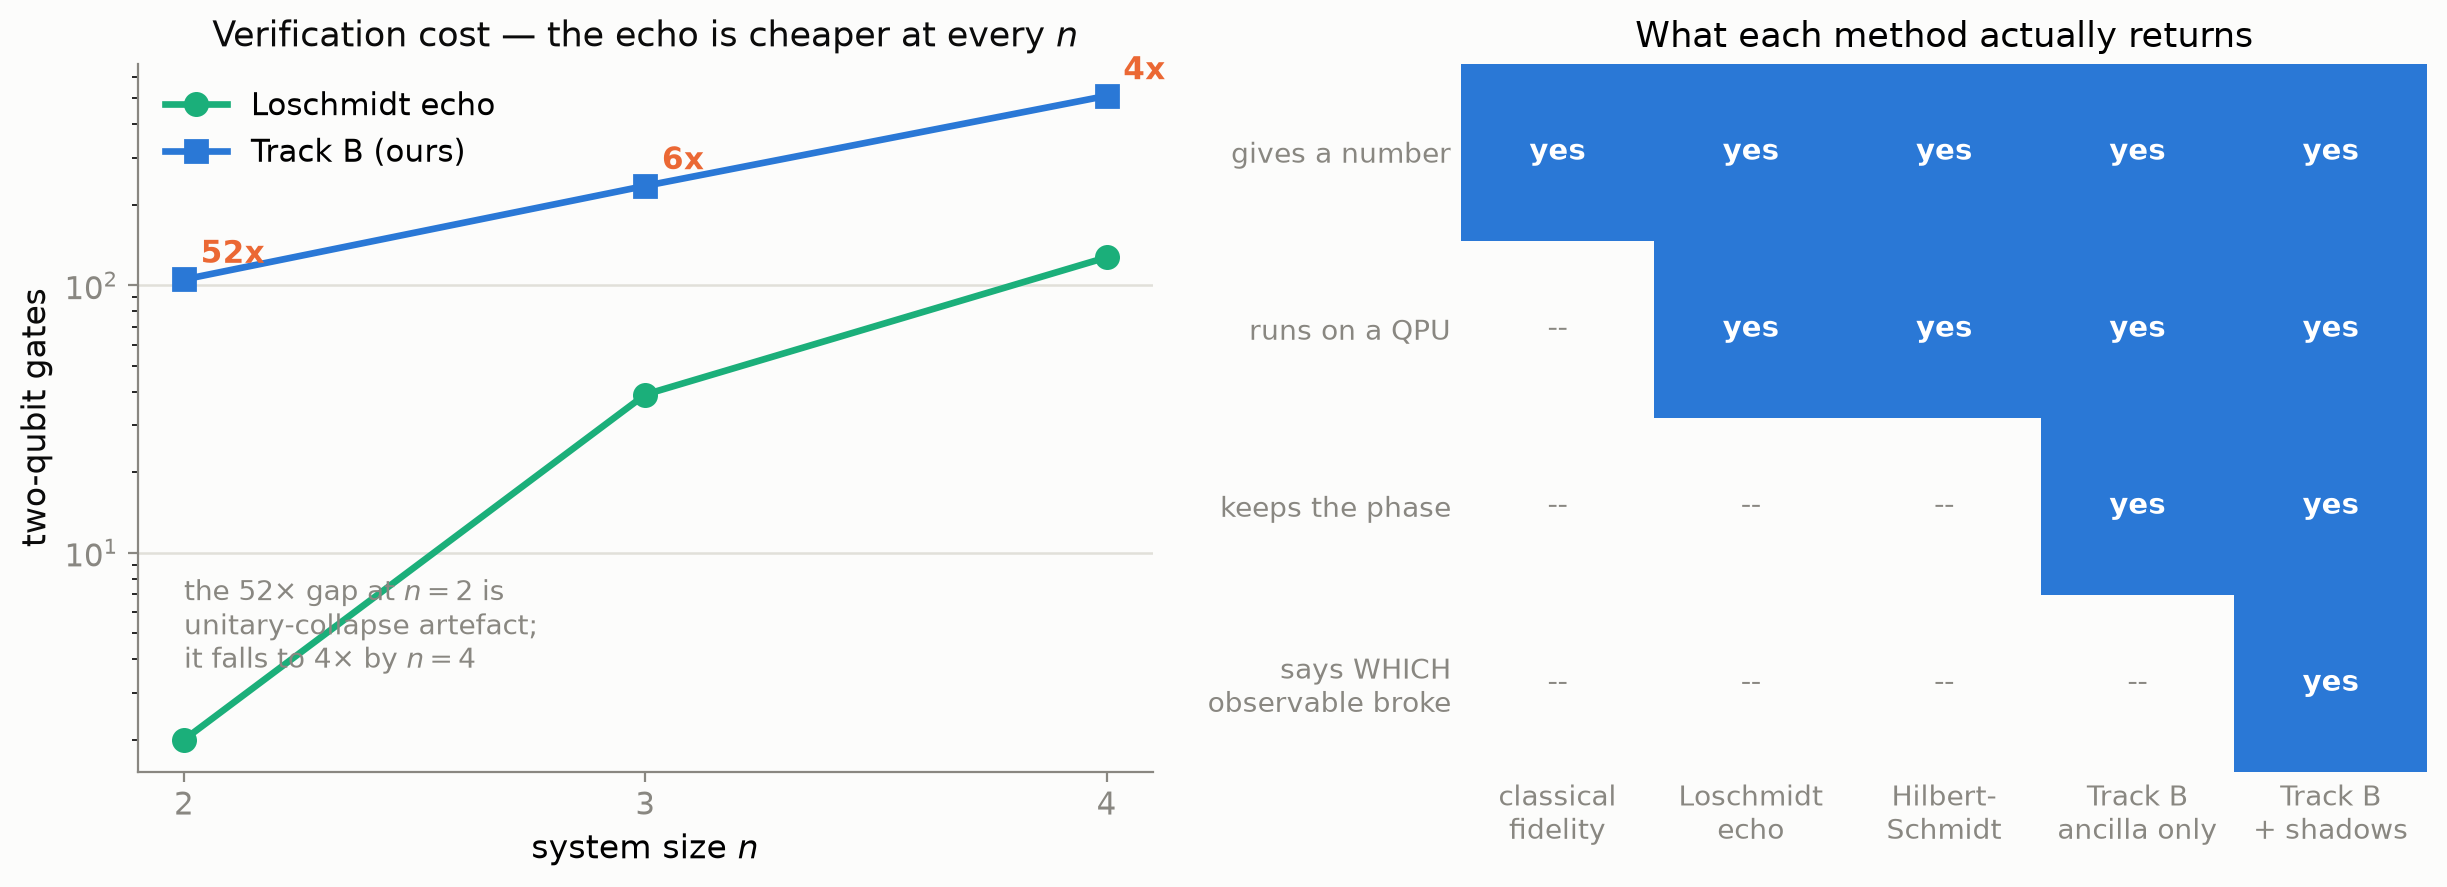
\includegraphics[width=0.99\linewidth]{fig_tb_baselines.png}
  \end{center}
  \vspace{-2mm}
  {\footnotesize
  \textbf{Loschmidt echo}: prepare, apply $U$, apply $W^\dagger$, un-prepare, read the
  all-zeros probability. \textbf{Hilbert--Schmidt test} (Khatri \emph{et al.},
  \emph{Quantum} \textbf{3}, 140 (2019)): Bell pairs on $2n$ qubits give the
  \emph{state-independent} $|\mathrm{Tr}[W^\dagger U]/d|^2$. Both verified against exact
  values before being used as baselines. \src{R043}}
\end{frame}

\begin{frame}{The honest scoreboard}
  \footnotesize
  \begin{center}
  \begin{tabular}{lccccc}
    \toprule
    & \textbf{qubits} & \textbf{2q gates} & \textbf{phase?} & \textbf{state-indep.?}
      & \textbf{which observable?}\\
    \midrule
    classical fidelity {\tiny(AQC's own score)} & --- & --- & n/a & yes & no\\
    Loschmidt echo        & $n$   & \good{2}  & no  & no  & no\\
    Hilbert--Schmidt test & $2n$  & 16        & no  & \good{yes} & no\\
    Track B, ancilla only & $n{+}1$ & 136     & \good{yes} & no & no\\
    Track B $+$ shadows {\tiny(ours)} & $n{+}1$ & 136 & \good{yes} & no & \good{yes}\\
    \bottomrule
  \end{tabular}
  \end{center}
  \smallskip
  \small
  \begin{itemize}
    \item \bad{The echo is cheaper than us at every $n$ we measured} --- $6.0\times$ at
          $n{=}3$ and $4.0\times$ at $n{=}4$. If all you want is a scalar ``how close is
          $W$ to $U$'', \emph{use the echo}. \src{R043}
    \item The $52\times$ gap at $n{=}2$ is a \emph{unitary-collapse artefact} (any product of
          2-qubit unitaries fuses into one). We quote 4--6$\times$, never 52$\times$.
    \item The HST answers a \emph{stronger} question than either overlap, and costs $2n$
          qubits for it.
  \end{itemize}
  \centering\textbf{Our arm has to be justified by what it returns, never by being cheaper.}
\end{frame}

% ==================================================================
\section{AQC: the compressor and its certificate}

\begin{frame}{AQC compression, certified by our own Track-B observable}
  \small
  Approximate Quantum Compiling (\texttt{qiskit-addon-aqc-tensor}, quimb$+$jax MPS backend)
  optimises a shallow ansatz against an MPS target. It scores itself with a
  \emph{classical} fidelity --- the one number you lose access to at scale.
  \medskip

  \begin{center}
  Set $W=$ the AQC circuit and $U=$ exact: then
  \hl{$\chi_{AB}=\langle\psi|W^\dagger U|\psi\rangle$ \emph{is} the compression fidelity},
  measured from shots.
  \end{center}
  \medskip

  \begin{center}
  \begin{tabular}{lccc}
    \toprule
    & \textbf{Trotter} & \textbf{exact synth.} & \textbf{AQC}\\
    \midrule
    \emph{uncontrolled} $n{=}3$ (infid. $1.4\!\times\!10^{-4}$) & 68 & 19 & \good{9}\\
    \emph{uncontrolled} $n{=}4$ (infid. $2.6\!\times\!10^{-4}$) & 104 & 95 & \good{15}\\
    \midrule
    \emph{controlled} $n{=}3$ --- what a Hadamard test runs & --- & \good{50} & \bad{132}\\
    \emph{controlled} $n{=}4$ & --- & 236 & \good{216}\\
    \bottomrule
  \end{tabular}
  \end{center}
  \smallskip
  {\footnotesize The compressor and the certificate come from two different halves of this
  project. \bad{But the story reverses under control:} at $n{=}3$ AQC is $2.6\times$
  \emph{worse}, because controlling an ansatz pays overhead on every gate while the direct
  block construction pays none. Crossover sits at $n\!\sim\!4$. \src{R035}}
\end{frame}

% ==================================================================
\section{On real hardware}

\begin{frame}{First Track B on a QPU --- and the cheap baseline beat us}
  \vspace{-1mm}
  \begin{center}
    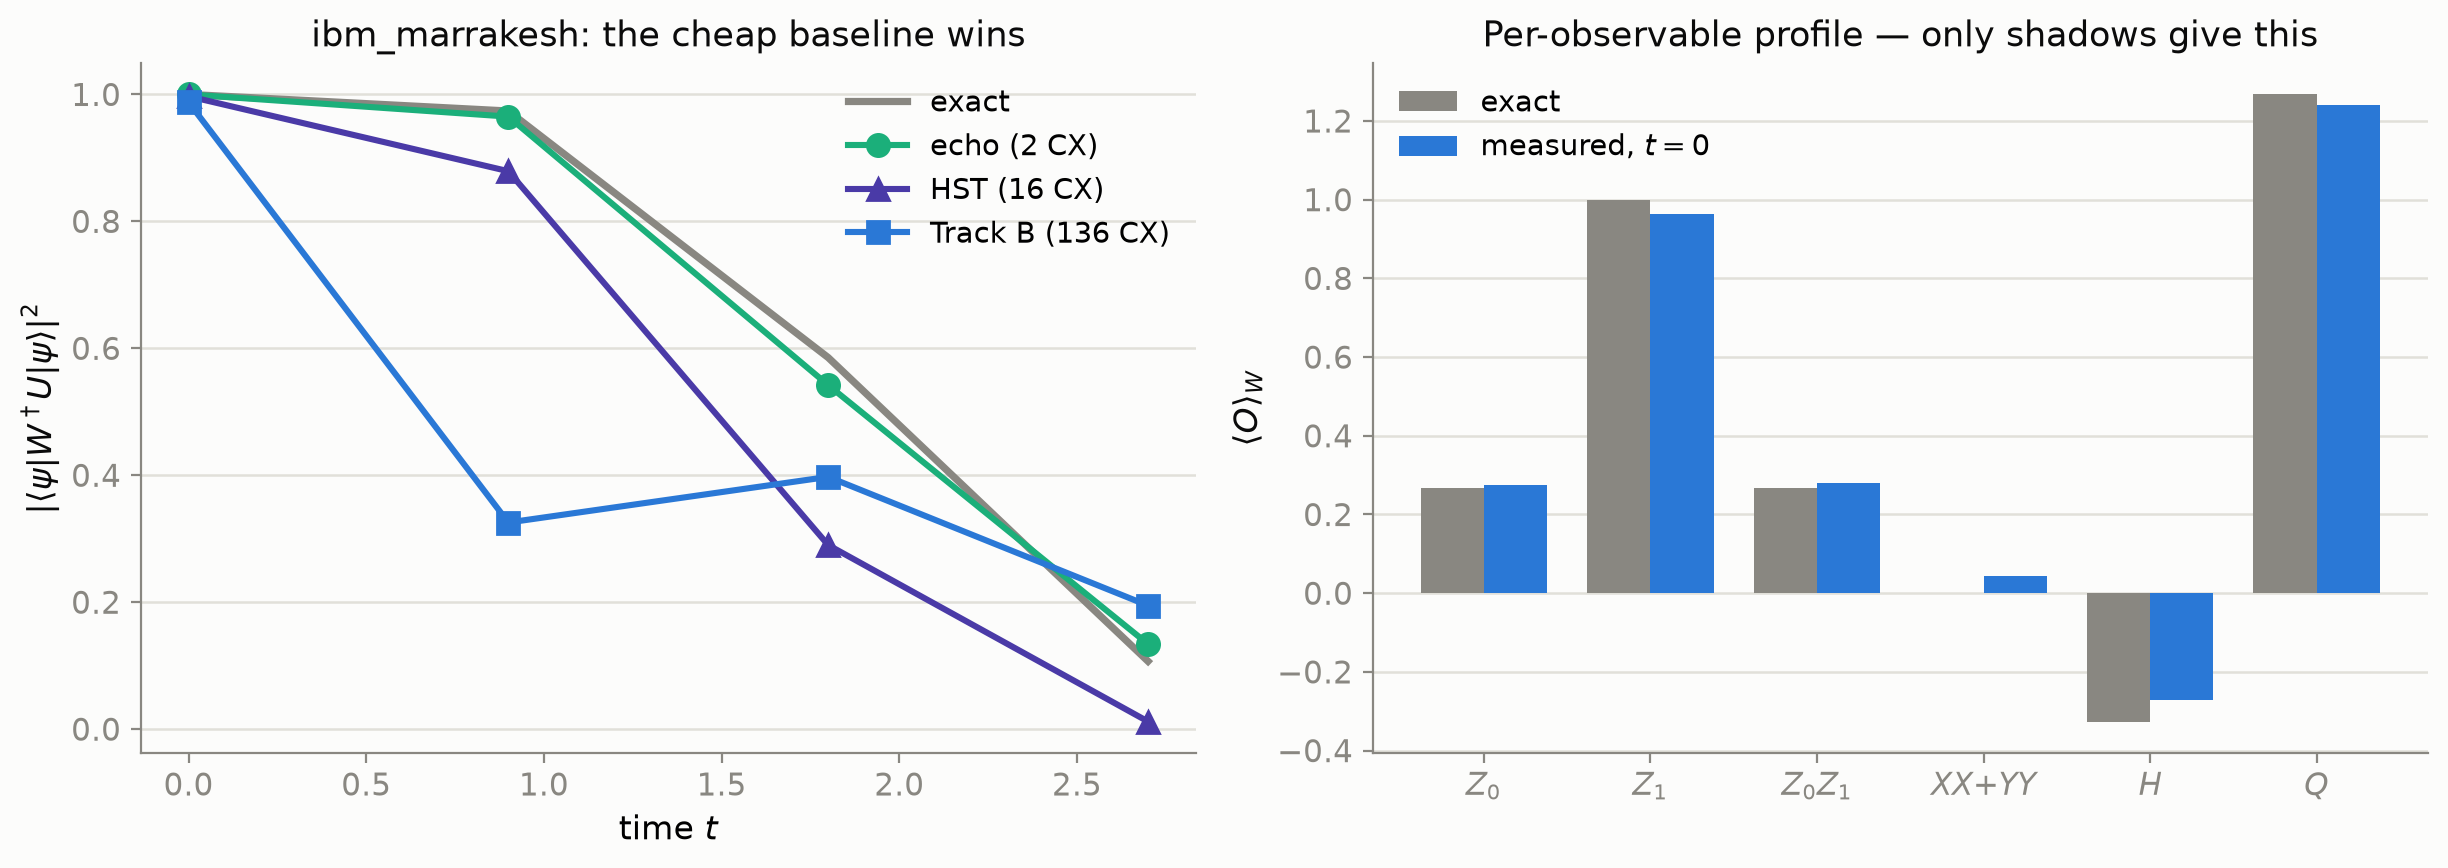
\includegraphics[width=0.99\linewidth]{fig_tb_hardware.png}
  \end{center}
  \vspace{-2mm}
  {\footnotesize
  \texttt{ibm\_marrakesh}, 116 circuits $\times$ 1000 shots, all four arms in \emph{one} job
  so the comparison is same-device same-hour. Predictions were recorded before submission.
  \bad{The 136-CX Track-B arm degrades fast:} clean at $t=0$ (errors all $\leq 0.053$), noise
  dominated by $t=0.9$. The 2-CX echo tracks the exact curve to $\sim\!0.04$ throughout.
  \src{R044}}
\end{frame}

\begin{frame}{The garbage also ships a free error bar}
  \begin{columns}[T]
    \begin{column}{0.54\textwidth}
      \centering
      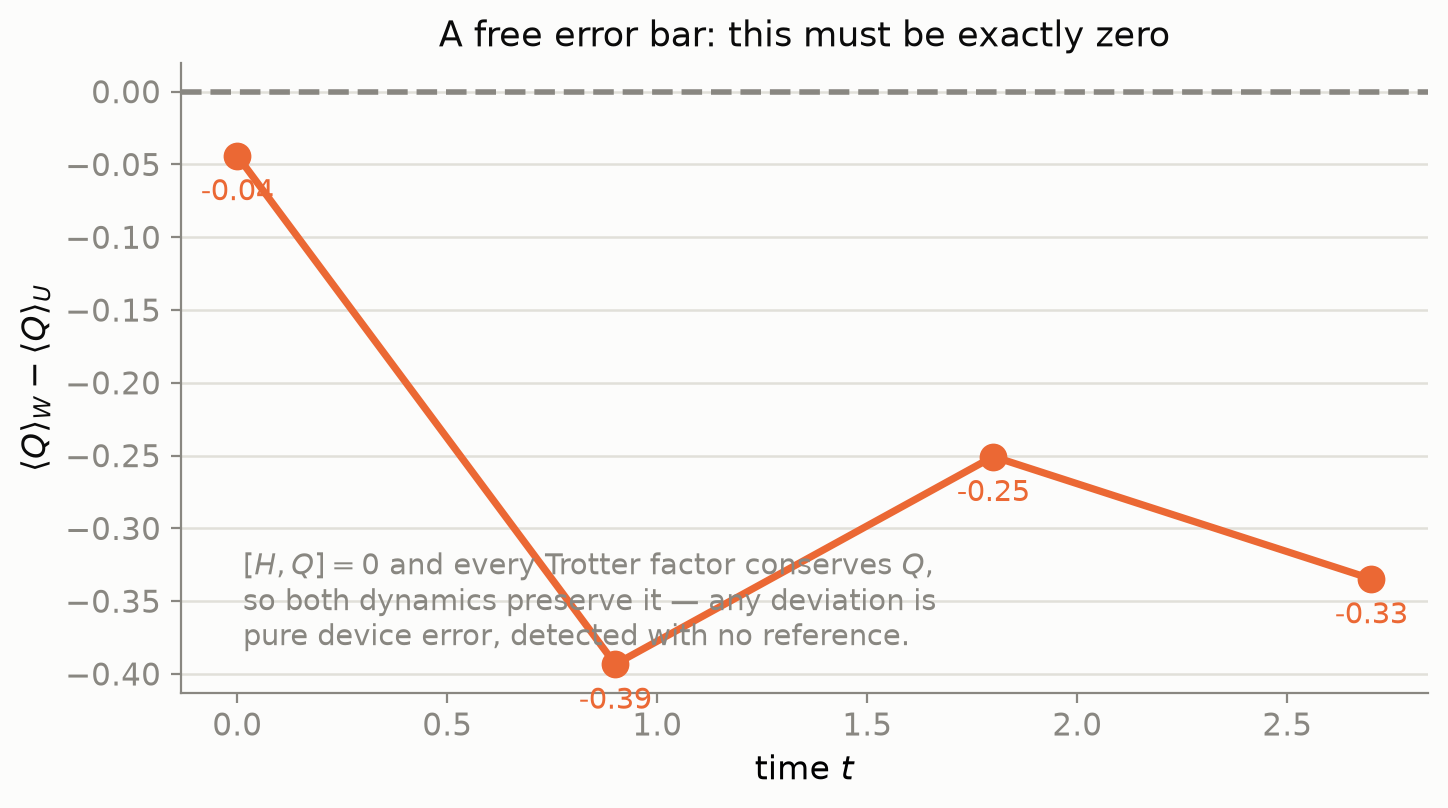
\includegraphics[width=\linewidth]{fig_tb_symmetry.png}
    \end{column}
    \begin{column}{0.44\textwidth}
      \small
      $Q=\sum_j Z_j$ commutes with $H$, and \emph{every} Trotter factor conserves it --- so
      $\langle Q\rangle_W-\langle Q\rangle_U$ is \hl{exactly zero} for any $W$ in this family.
      \medskip

      Measured: $-0.04$, $-0.39$, $-0.25$, $-0.34$. \src{R044}
      \medskip

      That deviation is \good{pure device error, detected with no reference state, no exact
      diagonalisation and no simulation} --- and it correctly flags the same times where the
      other observables went bad.
      \medskip

      {\footnotesize\color{mutedA} It is a diagnostic, not a correction: we do \emph{not}
      post-select on it, which would bias the shadow estimators.}
    \end{column}
  \end{columns}
\end{frame}

% ==================================================================
\section{What we claim}

\begin{frame}{What we claim, and what we do not}
  \small
  \textbf{We claim}
  \begin{itemize}
    \item Track B \hl{completed}: the per-observable disagreement profile via the X-basis
          readout, which our own R034 left undone. Identity validated to $4\times10^{-15}$
          on two models. \src{R042}
    \item An AQC-compressed circuit \hl{certified by a shot-based observable} rather than a
          classical fidelity --- the certificate survives to sizes where the classical score
          does not. \src{R035}
    \item Track B run on a \hl{QPU for the first time in this project}, against two
          literature baselines in the same job. \src{R044}
  \end{itemize}
  \medskip
  \textbf{We do not claim}
  \begin{itemize}
    \item \bad{That our method is the best way to get the scalar overlap.} It is not --- the
          Loschmidt echo is 4--6$\times$ cheaper and, on hardware, markedly more accurate.
    \item \bad{That AQC helps a Hadamard test at these sizes.} Under control it is
          $2.6\times$ worse at $n{=}3$; the crossover is at $n\!\sim\!4$. \src{R035}
    \item Any advantage over classical computation. The instance is 2--3 qubits and a laptop
          solves it exactly --- which is the point: every number here is graded against truth.
  \end{itemize}
\end{frame}

\begin{frame}{Reproduce it}
  \small
  \begin{itemize}
    \item \texttt{evidence/scripts/track\_b\_ab\_tester.py} --- Track B derivation
          $+$ statevector validation $+$ simulator study \src{R034}
    \item \texttt{evidence/scripts/track\_b\_baselines.py} --- Loschmidt echo, Hilbert--Schmidt
          test, and the $n{=}2,3,4$ cost scaling \src{R043}
    \item \texttt{evidence/scripts/track\_b\_hardware\_submit.py} --- validate-then-submit,
          all four arms; refuses to submit if the identity check fails \src{R042}
    \item \texttt{evidence/scripts/track\_b\_hardware\_fetch.py} --- the analysis behind
          every hardware number on these slides \src{R044}
    \item \texttt{evidence/scripts/aqc\_compression.py} --- AQC $+$ Track-B certification
          \src{R035}
  \end{itemize}
  \vfill
  \centering
  \Large\textbf{Garbage Collectors}\\
  \normalsize Thank you --- questions welcome.
\end{frame}

\end{document}
